\subsection*{Supplementary information [Not applicable]}

\subsubsection*{Observation formulation of GridSim}
As shown in Extended Table.1, the observation is a dictionary of different values, including time, generator states, load states, line status and ultra-short-term forecasts.
\begin{table}[h]
    \centering
    \begin{tiny}
    \begin{tabular}{ccc}
    \toprule
        Variable Name & Data Type & Meaning \\
    \midrule
        timestep & int & current steps \\
        vTime & string & current timestamp \\
        gen\_p & list[float] & active power of generators \\
        gen\_q & list[float] & reactive power of generators \\
        gen\_v & list[float] & voltage magnitudes of generators \\
        load\_p & list[float] & active power of loads \\
        load\_q & list[float] & reactive power of loads \\
        load\_v & list[float] & voltage magnitudes of loads \\
        line\_status & list[bool] & line status \\
        grid\_loss & float & transmission loss \\
        action\_space & dict & legal action space of the next step\\
        rho & list[float] & line load rate\\
        gen\_status & list[bool] & generator status, 1-on/0-off \\
        steps\_to\_recover\_gen & np.ndarray & number of steps for closed units to restart \\
        steps\_to\_close\_gen & np.ndarray & number of steps for restarted units to shutdown \\
        curstep\_renewable\_gen\_p\_max & list[float] & max power of the renewable unit at the current step \\
        nextstep\_renewable\_gen\_p\_max & list[float] & max power of the renewable unit at the next step \\
        next\_load\_p & list[float] & load for the next step \\
    \bottomrule
    \end{tabular}
    \captionsetup{labelformat=empty}
    \caption{\textbf{Extended Table. 1:} Main components of $GridSim.observation$. Please refer to the supplementary data for more details.}
    \end{tiny}
    \label{tab:observation}
\end{table}

\subsubsection*{Action space formulation}
As shown in Extended Table.2, the action space is a dictionary of the upper boundaries and lower boundaries of generators' output power. For thermal generators, their upper bounds and lower bounds are determined as $[-\text{p}_\text{ramp}, \text{p}_\text{ramp}]$. For renewable generators, since their output power could be set as $[0,\overline{\text{p}}]$ at each step, their upper bounds and lower bounds are $[-\text{p}, \overline{\text{p}}-\text{p}]$.
\begin{table}[h]
    \centering
    \begin{tiny}
    \begin{tabular}{ccc}
    \toprule
        Variable Name & Data Type & Meaning \\
    \midrule
        % adjust\_gen\_p & np.ndarray & active power adjustments of generators \\
        adjust\_gen\_p.high & np.ndarray & upper bound of active power adjustment of generators\\
        adjust\_gen\_p.low & np.ndarray & lower bound of active power adjustment of generators\\
    \bottomrule
    \end{tabular}
    \captionsetup{labelformat=empty}
    \caption{\textbf{Extended Table. 2:} Main components of $GridSim.action\_space$. Please refer to the supplementary data for more details.}
    \end{tiny}
    \label{tab:observation}
\end{table}

\subsubsection*{Static parameters of GridSim}
Some static parameters of GridSim are shown in Extended Table.3, including the indexes of renewable generators, power ramping rate of thermal generators, etc. 
\begin{table}[h]
    \centering
    \begin{tiny}
    \begin{tabular}{ccc}
    \toprule
        Variable Name & Data Type & Meaning \\
    \midrule
        num\_gen & int & number of generators \\
        num\_line & int & number of lines \\ 
        num\_load & int & number of loads \\
        num\_bus & int & number of buses \\
        gen\_type & list[int] & generator types, 5-renewable, 1-thermal, 2-balanced\\
        max\_gen\_p & list[float] & upper bound of active power output \\
        min\_gen\_p & list[float] & lower bound of active power output \\
        max\_gen\_q & list[float] & upper bound of reactive power output \\
        min\_gen\_q & list[float] & lower bound of reactive power output \\
        max\_gen\_v & list[float] & upper bound of generator voltage magnitude \\
        min\_gen\_v & list[float] & lower bound of generator voltage magnitude \\
        ramp\_rate & float & active power ramping factor of thermal generators \\
        thermal\_ids & list[int] & thermal generators index \\
        renewable\_ids & list[int] & renewable generators index \\
        balanced\_id & list[int] & balanced generator index\\
        startup\_cost & list[float] & starup cost\\
        constant\_cost & list[float] & constant cost \\
        first\_order\_cost & list[float] & first order cost coefficient \\
        second\_order\_cost & list[float] & second order cost coefficient\\
    \bottomrule
    \end{tabular}
    \captionsetup{labelformat=empty}
    \caption{\textbf{Extended Table. 3:} Main components of $GridSim.static\_parameters$. Please refer to the supplementary data for more details.}
    \end{tiny}
    \label{tab:observation}
\end{table}

\subsubsection*{Rules of GridSim}
\paragraph{The upper and lower limits of the active output of the unit} The active power of any unit (except the balancing unit) cannot be greater than the upper limit of the active power, nor can it be smaller than the lower limit of the active power. If it is violated, the emulator prompts "illegal action", forcibly ending the episode.

\paragraph{Maximum output constraint of new energy units} 
In any time step, the active power output of renewable energy units cannot be greater than the maximum power generation capability. If it is violated, the emulator prompts "illegal action", forcibly ending the round.

\paragraph{Unit ramping constraint} The active power adjustment of any thermal power unit must be smaller than the ramping rate. If it is violated, the emulator prompts "illegal action", forcibly ending the episode.

\paragraph{Unit startup/shutdown constraints} The shutdown rule for thermal power units is that the active power output of the unit must be adjusted to the lower bound before the unit is shutdown, and then adjusted to 0. Restarting is not allowed within 40 consecutive steps after the unit is stopped. The startup rule of thermal power units is that the active power output must be adjusted to the lower bound before the unit is turned on. No shutdown is allowed for 40 consecutive time steps after the unit is restarted.

\paragraph{Line overflow constraint} If the line current exceeds the limit but does not exceed 135\% of the thermal limit, it means that the branch is "soft overloaded". If the line current exceeds 135\% of the thermal regulation limit, it means the line is "hard overloaded". If any line has "soft overload" for 4 consecutive time steps, the line will be shut down. In the event of a "hard overload", the line is immediately shut down. After the line has been out of service for 16 time steps, it will be put into operation again.

\paragraph{Upper and lower limit constraints of the unit's reactive power output} When the agent adjusts the voltage at the machine terminal, the unit's reactive power output value exceeds its upper and lower limits, and a negative reward will be obtained.
\paragraph{Voltage upper and lower limit constraints} If the node voltage exceeds its upper and lower limits, it will get a negative reward.

\paragraph{Upper and lower limit constraints of the balancing machine} The system sets a balancing unit to share the unbalanced power of the system caused by the unreasonable control strategy. After the power flow calculation, if the active power output of the balancing unit is greater than the upper limit but less than 110\% of the upper limit, or less than the lower limit but greater than 90\% of the lower limit, a negative reward will be obtained. If the output is greater than 110\% of the upper limit or less than 90\% of the lower limit, the episode ends.

\subsubsection*{Training statistics}
As shown in Extended Fig.1, GridZero much outperforms SAC, which shows the superiority of planning over the actor-critic framework in terms of policy improvement. All experiments are done on a machine with 8 Nvidia RTX-2080Ti GPUs and 80 cores of Intel Xeon Gold 5218R CPU.

\begin{figure}[h]
\centering
% \begin{minipage}[t]{0.6\linewidth}
% \centering
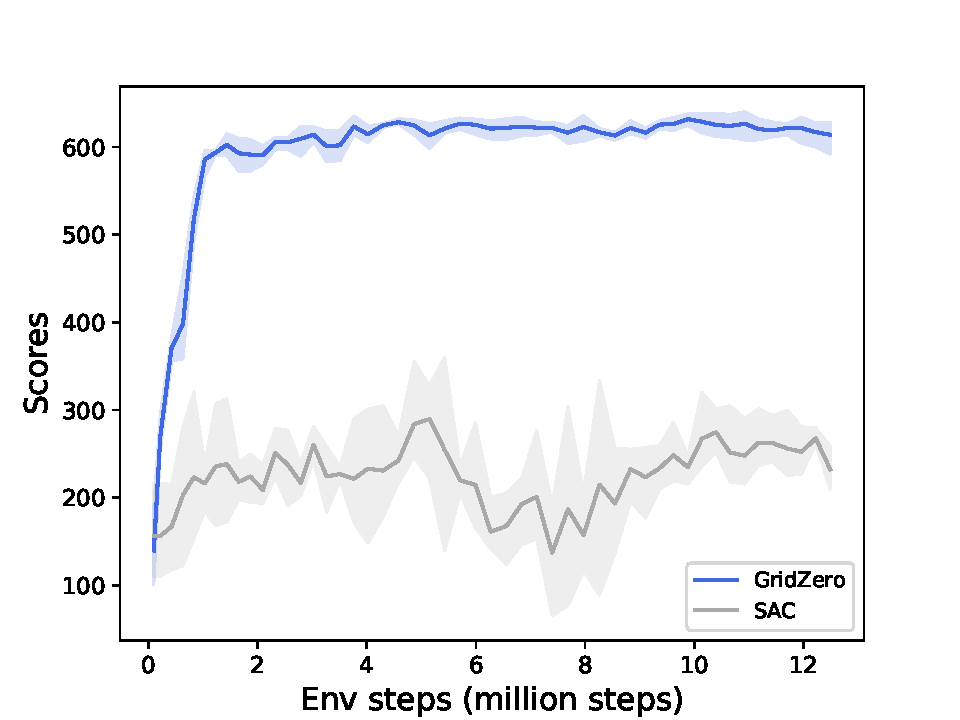
\includegraphics[width=0.6\linewidth]{fig/performance_curve.pdf}
\captionsetup{labelformat=empty}
% \end{minipage}
\caption{\textbf{Extended Fig. 1:}
Performance curves of GridZero and SAC. The X-axis represents environmental steps. The Y-axis indicates the average episode scores. GridZero much outperforms the model-free baseline SAC. The average scores among 20 evaluation seeds for 4 runs is shown on the Y-axis. }
\label{fig:perf-sns-trade-off}
\end{figure}

Moreover, Extended Fig.1 and Extended Fig.2 both show that GridZero is highly sample-efficient that it only requires 1 million environmental interaction steps and 15-kilo training steps.
\begin{figure}[h]
    \centering
    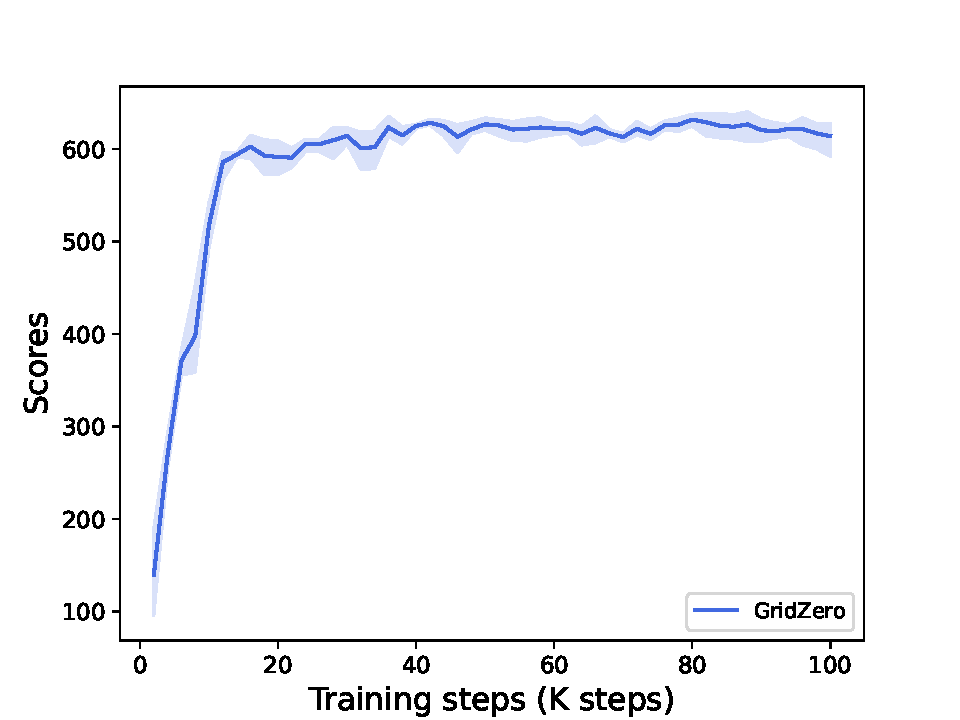
\includegraphics[width=0.6\linewidth]{fig/perfmance_trainsteps.pdf}
    \captionsetup{labelformat=empty}
    \caption{\textbf{Extended Fig. 2:} Training curves of GridZero. X-axis represents training steps. Y-axis indicates episode scores. The average scores among 20 evaluation seeds for 4 runs is shown on the Y-axis.}
    \label{fig:perf_training}
\end{figure}

Extended Fig.3 shows GridZero's performance in 20 different scenarios. In each scenario, GridZero significantly reduces renewable curtailment, and keeps the adjustment capacity area well covering the load curve.
\begin{figure}[h]
  \centering
  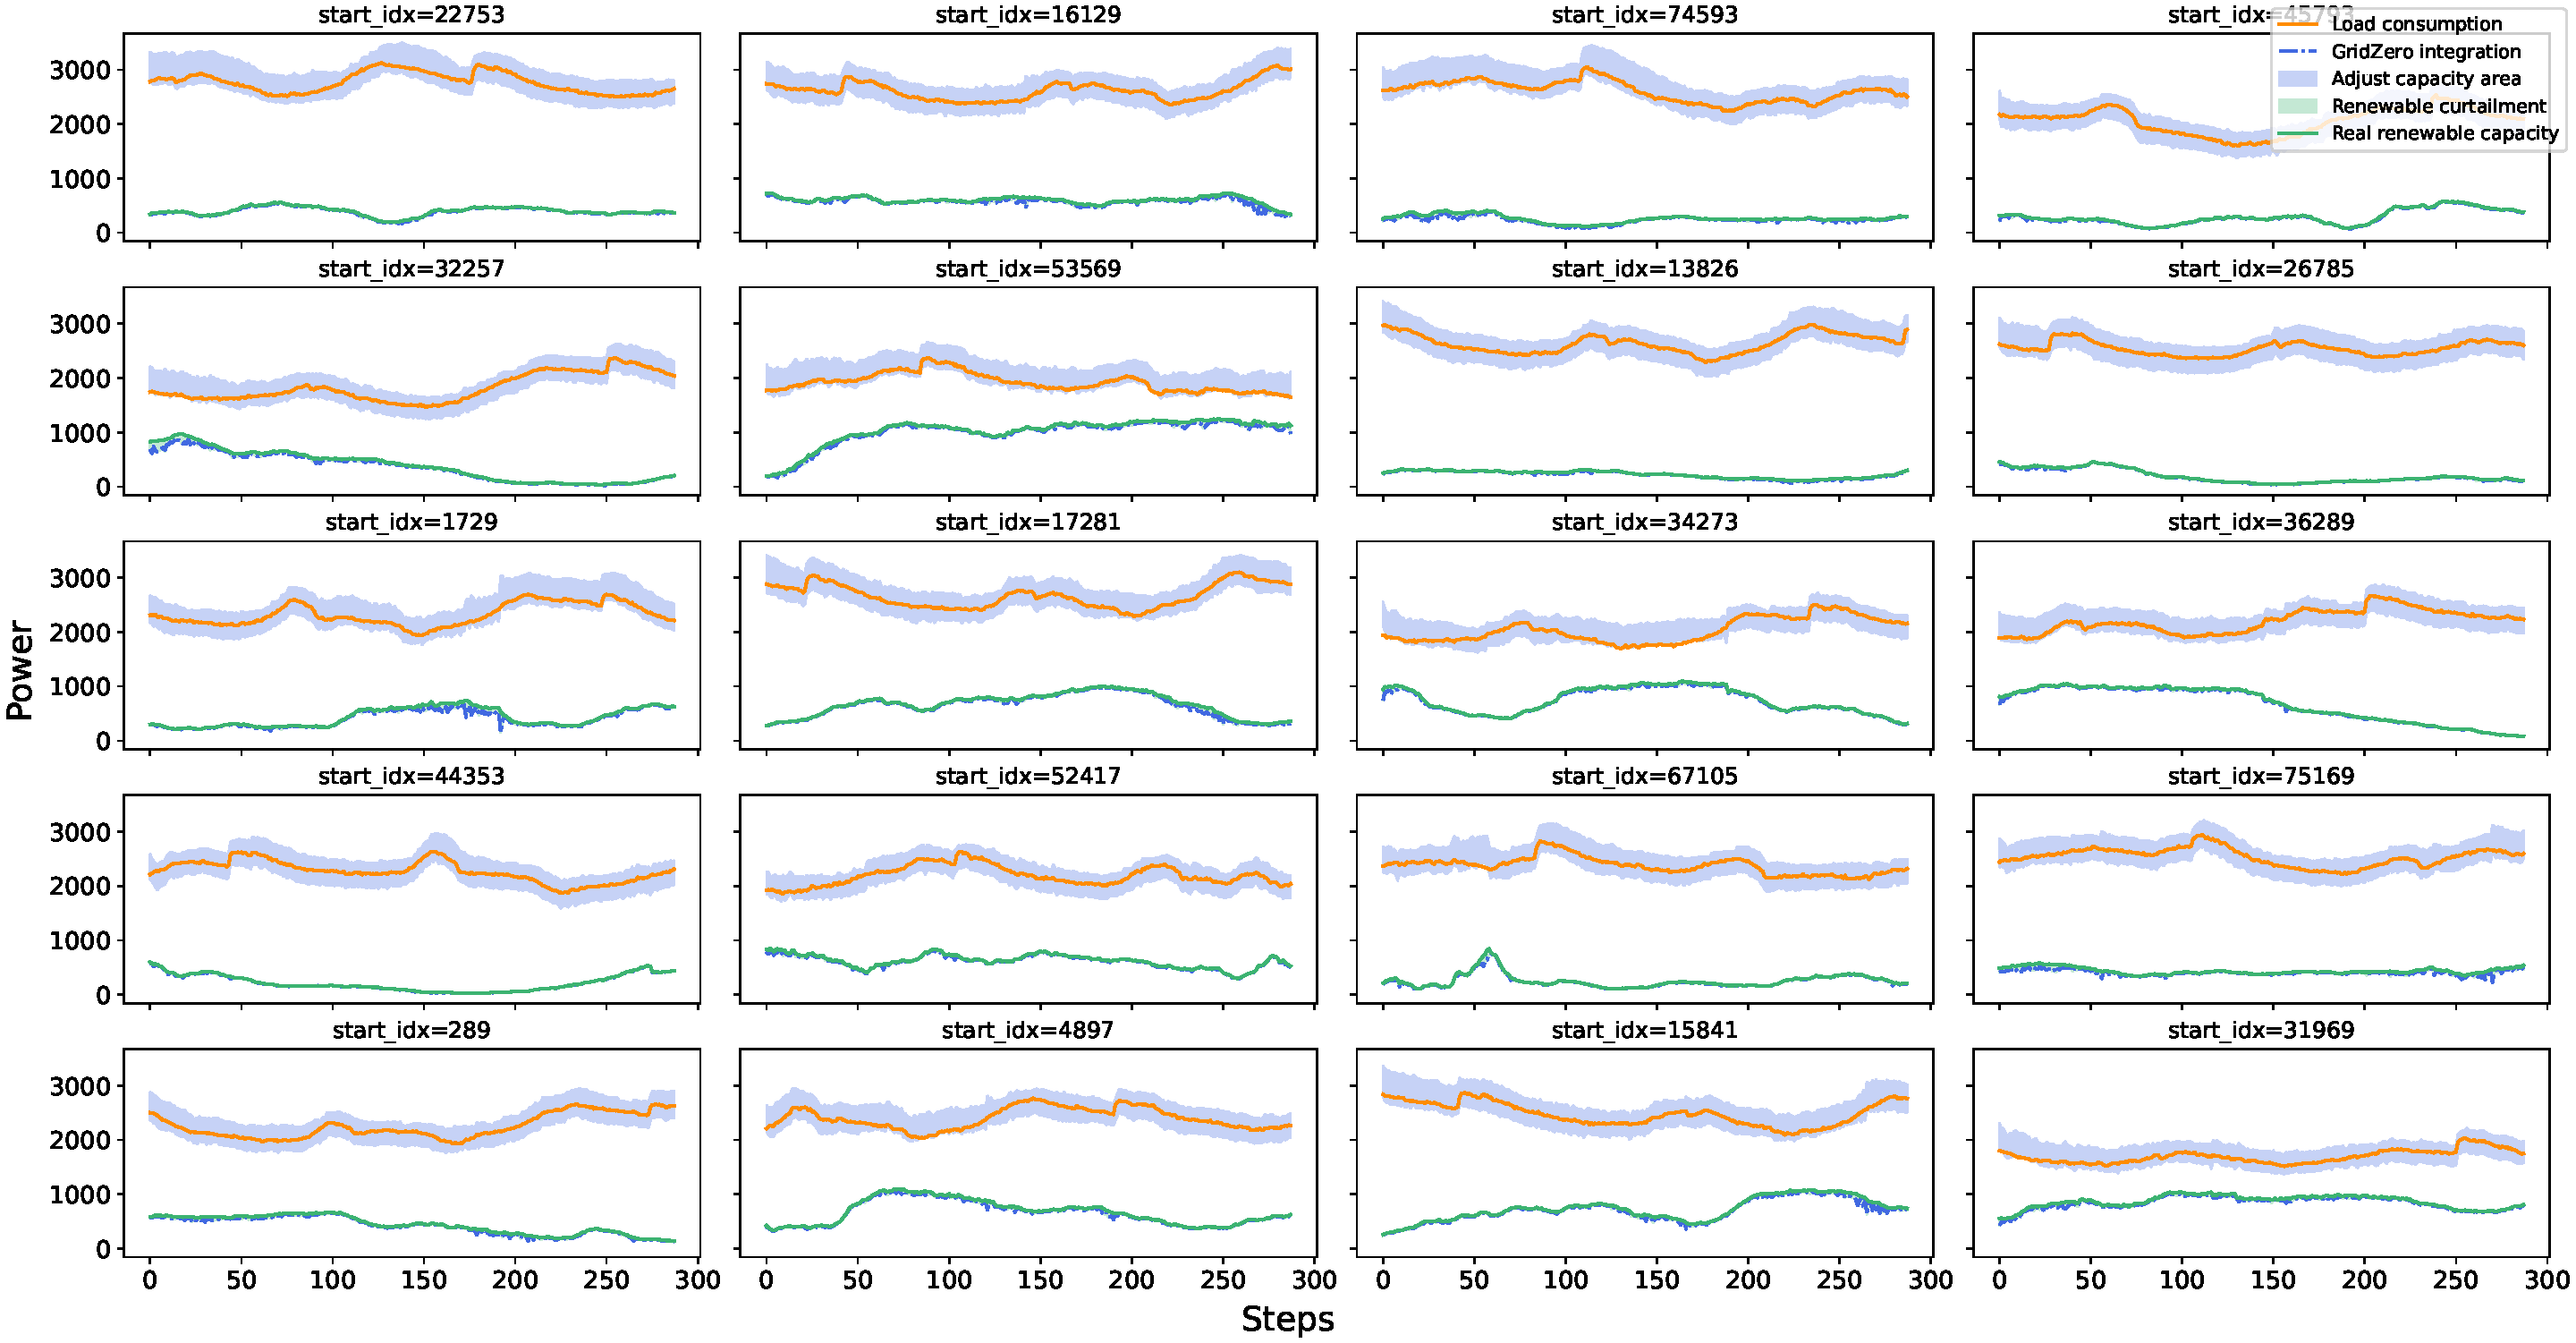
\includegraphics[width=1.0\linewidth]{fig/20_episodes.pdf}
  \captionsetup{labelformat=empty}
  \caption{\textbf{Extended Fig. 3:} Renewable consumption and load curves of 20 test scenarios. X-axis represents 288 dispatching steps over a whole day. Y-axis indicates power. GridZero could well track maximum power curve of renewable sources and keep the adjust capacity area covering the load consumption curve. 
  % In renewable energy rich scenarios, such as section 53569, GridZero can adjust the on-off status of thermal units to bring as much "green electricity" onto the grid as possible. GridZero achieves similar performance to AC-OPF in renewable energy consumption. The early plunge to 0 of curves of SAC and DDPG means that those model-free agents caonnot run the whole episode.
  } 
  \label{fig:20_episodes}
\end{figure}

Extended Fig.4 shows the learning process of different constraints, the operation cost and the renewable consumption rate. All constraint violation rates decrease with the training process, also including the operation cost. GridZero also achieves 95\% of an average renewable consumption rate.
\begin{figure}[h]
    \centering
    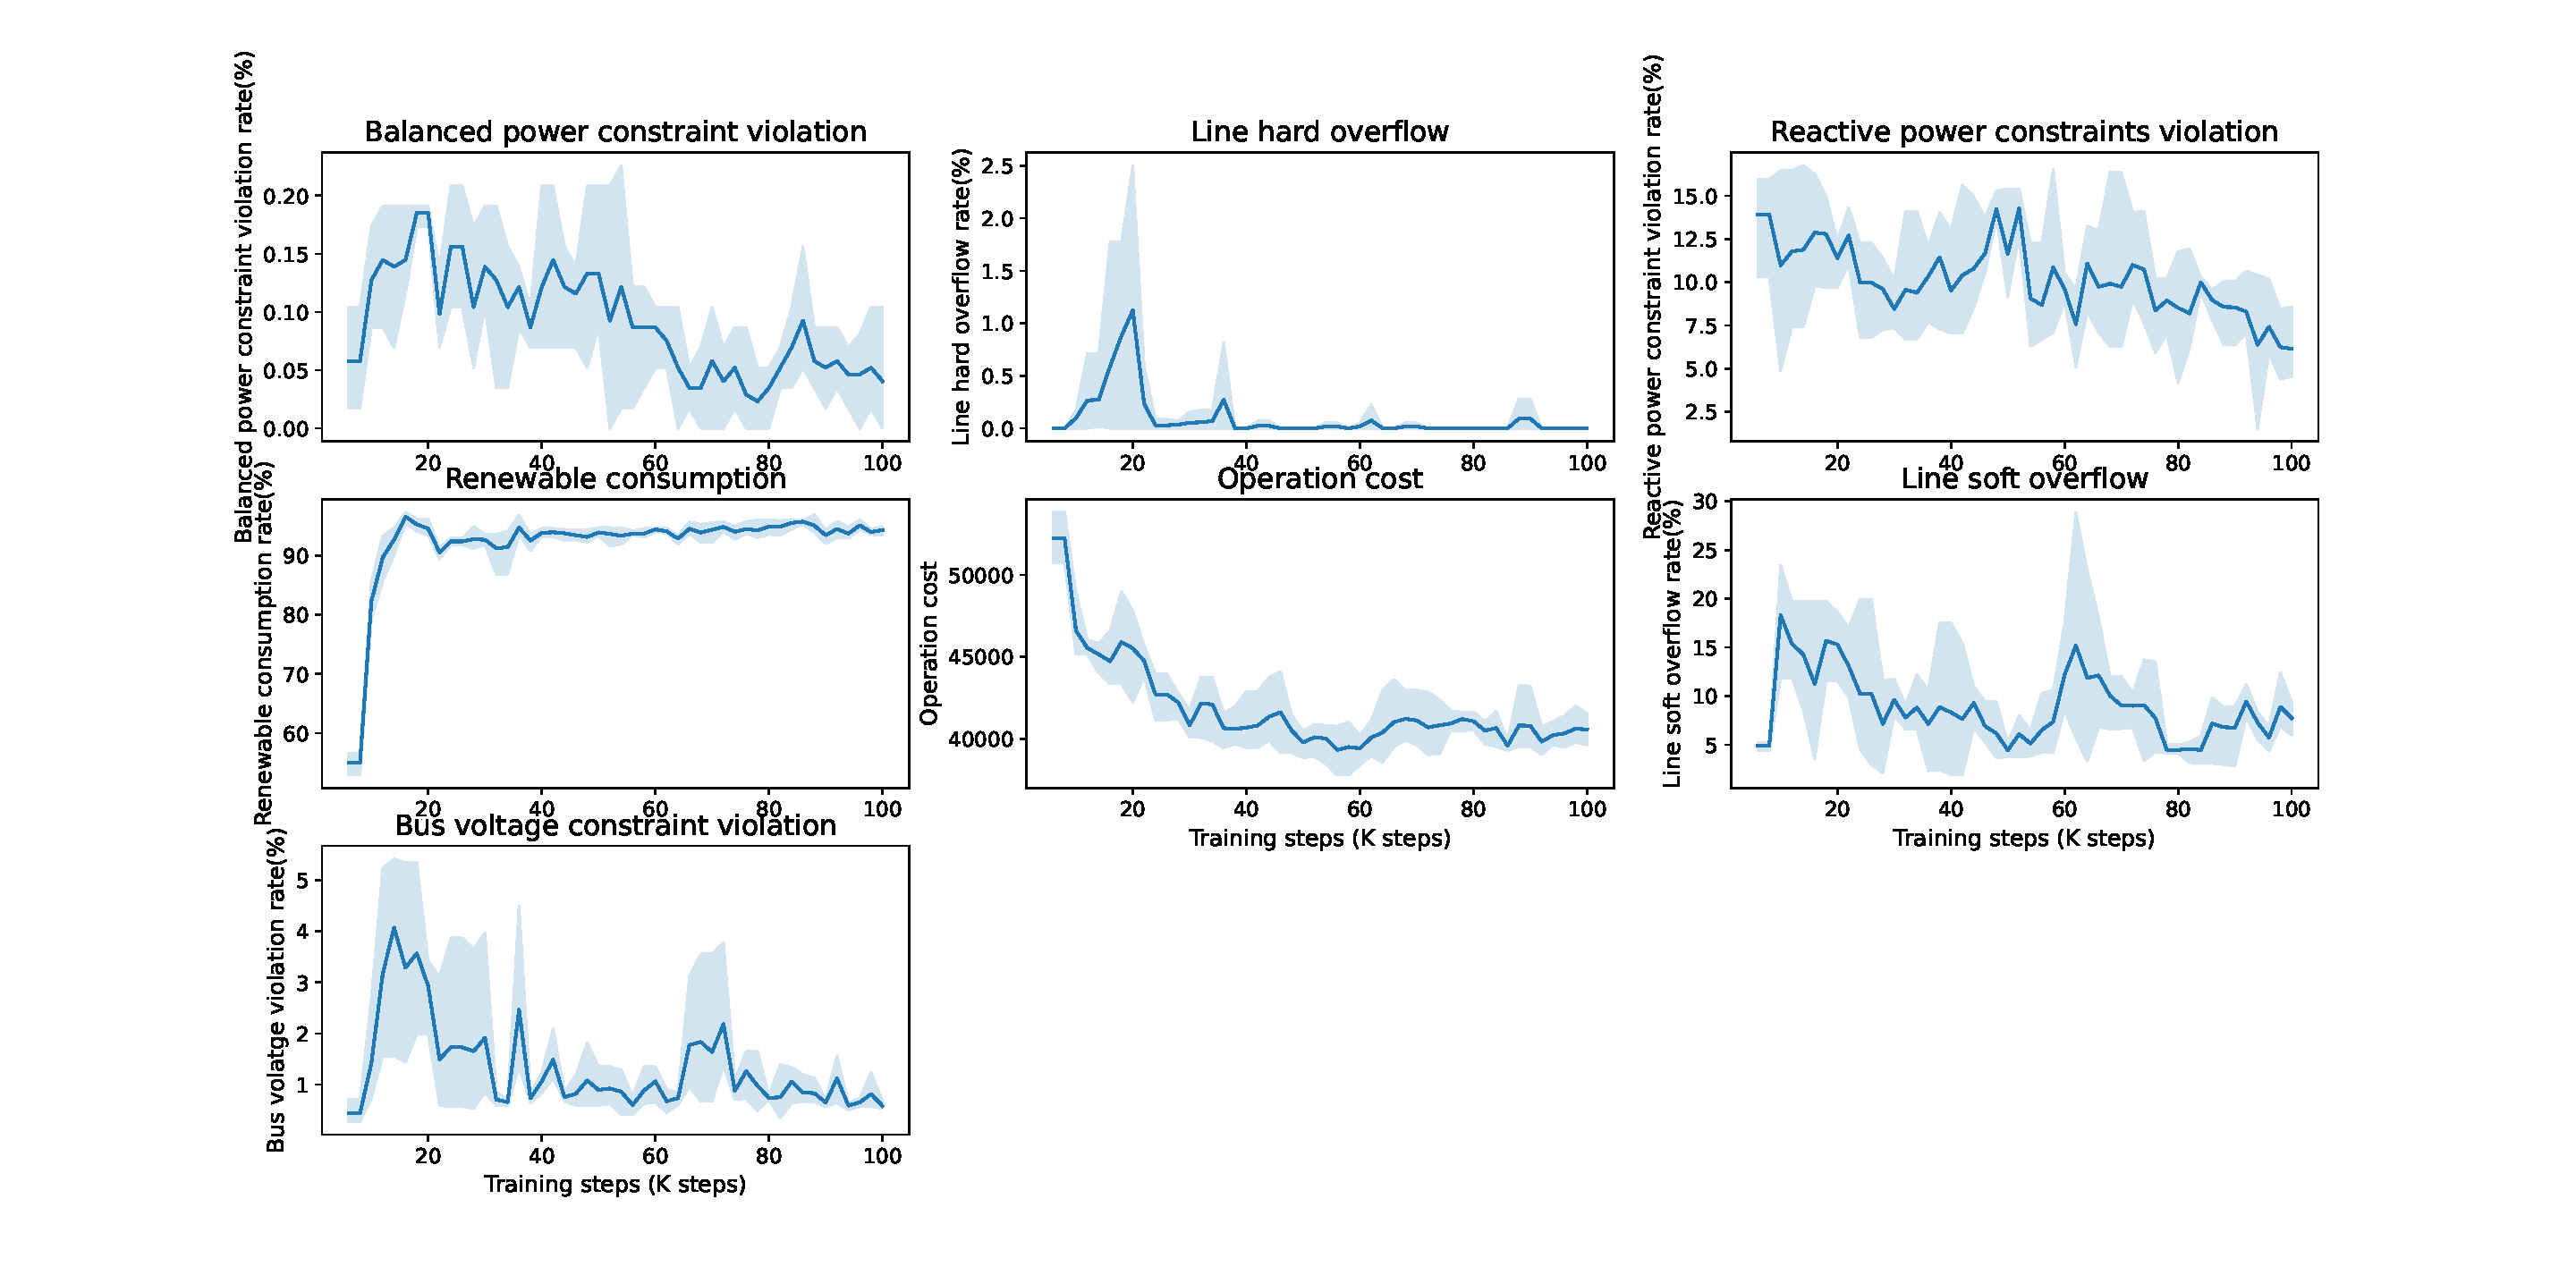
\includegraphics[width=1.0\linewidth]{fig/constraint_learning.pdf}
    \captionsetup{labelformat=empty}
    \caption{\textbf{Extended Fig. 4:} Learning curves of constraints and objectives. X-axis represents the training steps. Y-axis represents the violation rates or objective values.}
    \label{fig:my_label}
\end{figure}

\subsubsection*{Network architecture}
As shown in  Extended Fig.5, since RTS is a state-based task. All of our networks are implemented by simple Multi-Layer Perceptron (MLP). The more complex network architectures, such as Graph Neural Networks (GNN), could be further studied in future works.
\begin{figure}[h]
    \centering
    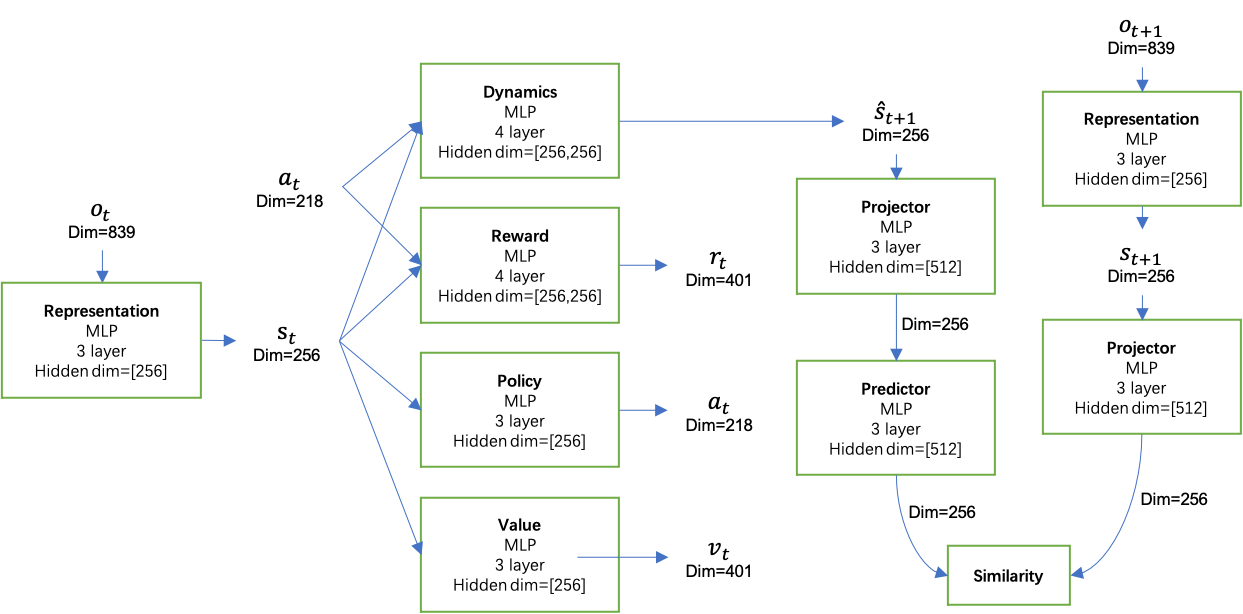
\includegraphics[width=1.0\linewidth]{fig/net_arch.png}
    \captionsetup{labelformat=empty}
    \caption{\textbf{Extended Fig. 5:} Network architecture of GirdZero. All sub-networks are MLPs.}
    \label{fig:net_arch}
\end{figure}

\subsubsection*{Power Grid Architecture}
The power grid architecture is shown in Extended Fig.6, including 126 buses, 185 lines, 54 generators, and 91 loads. This provincial grid is divided into three sub-networks, scattered in different areas.
\begin{figure}[h]
    \centering
    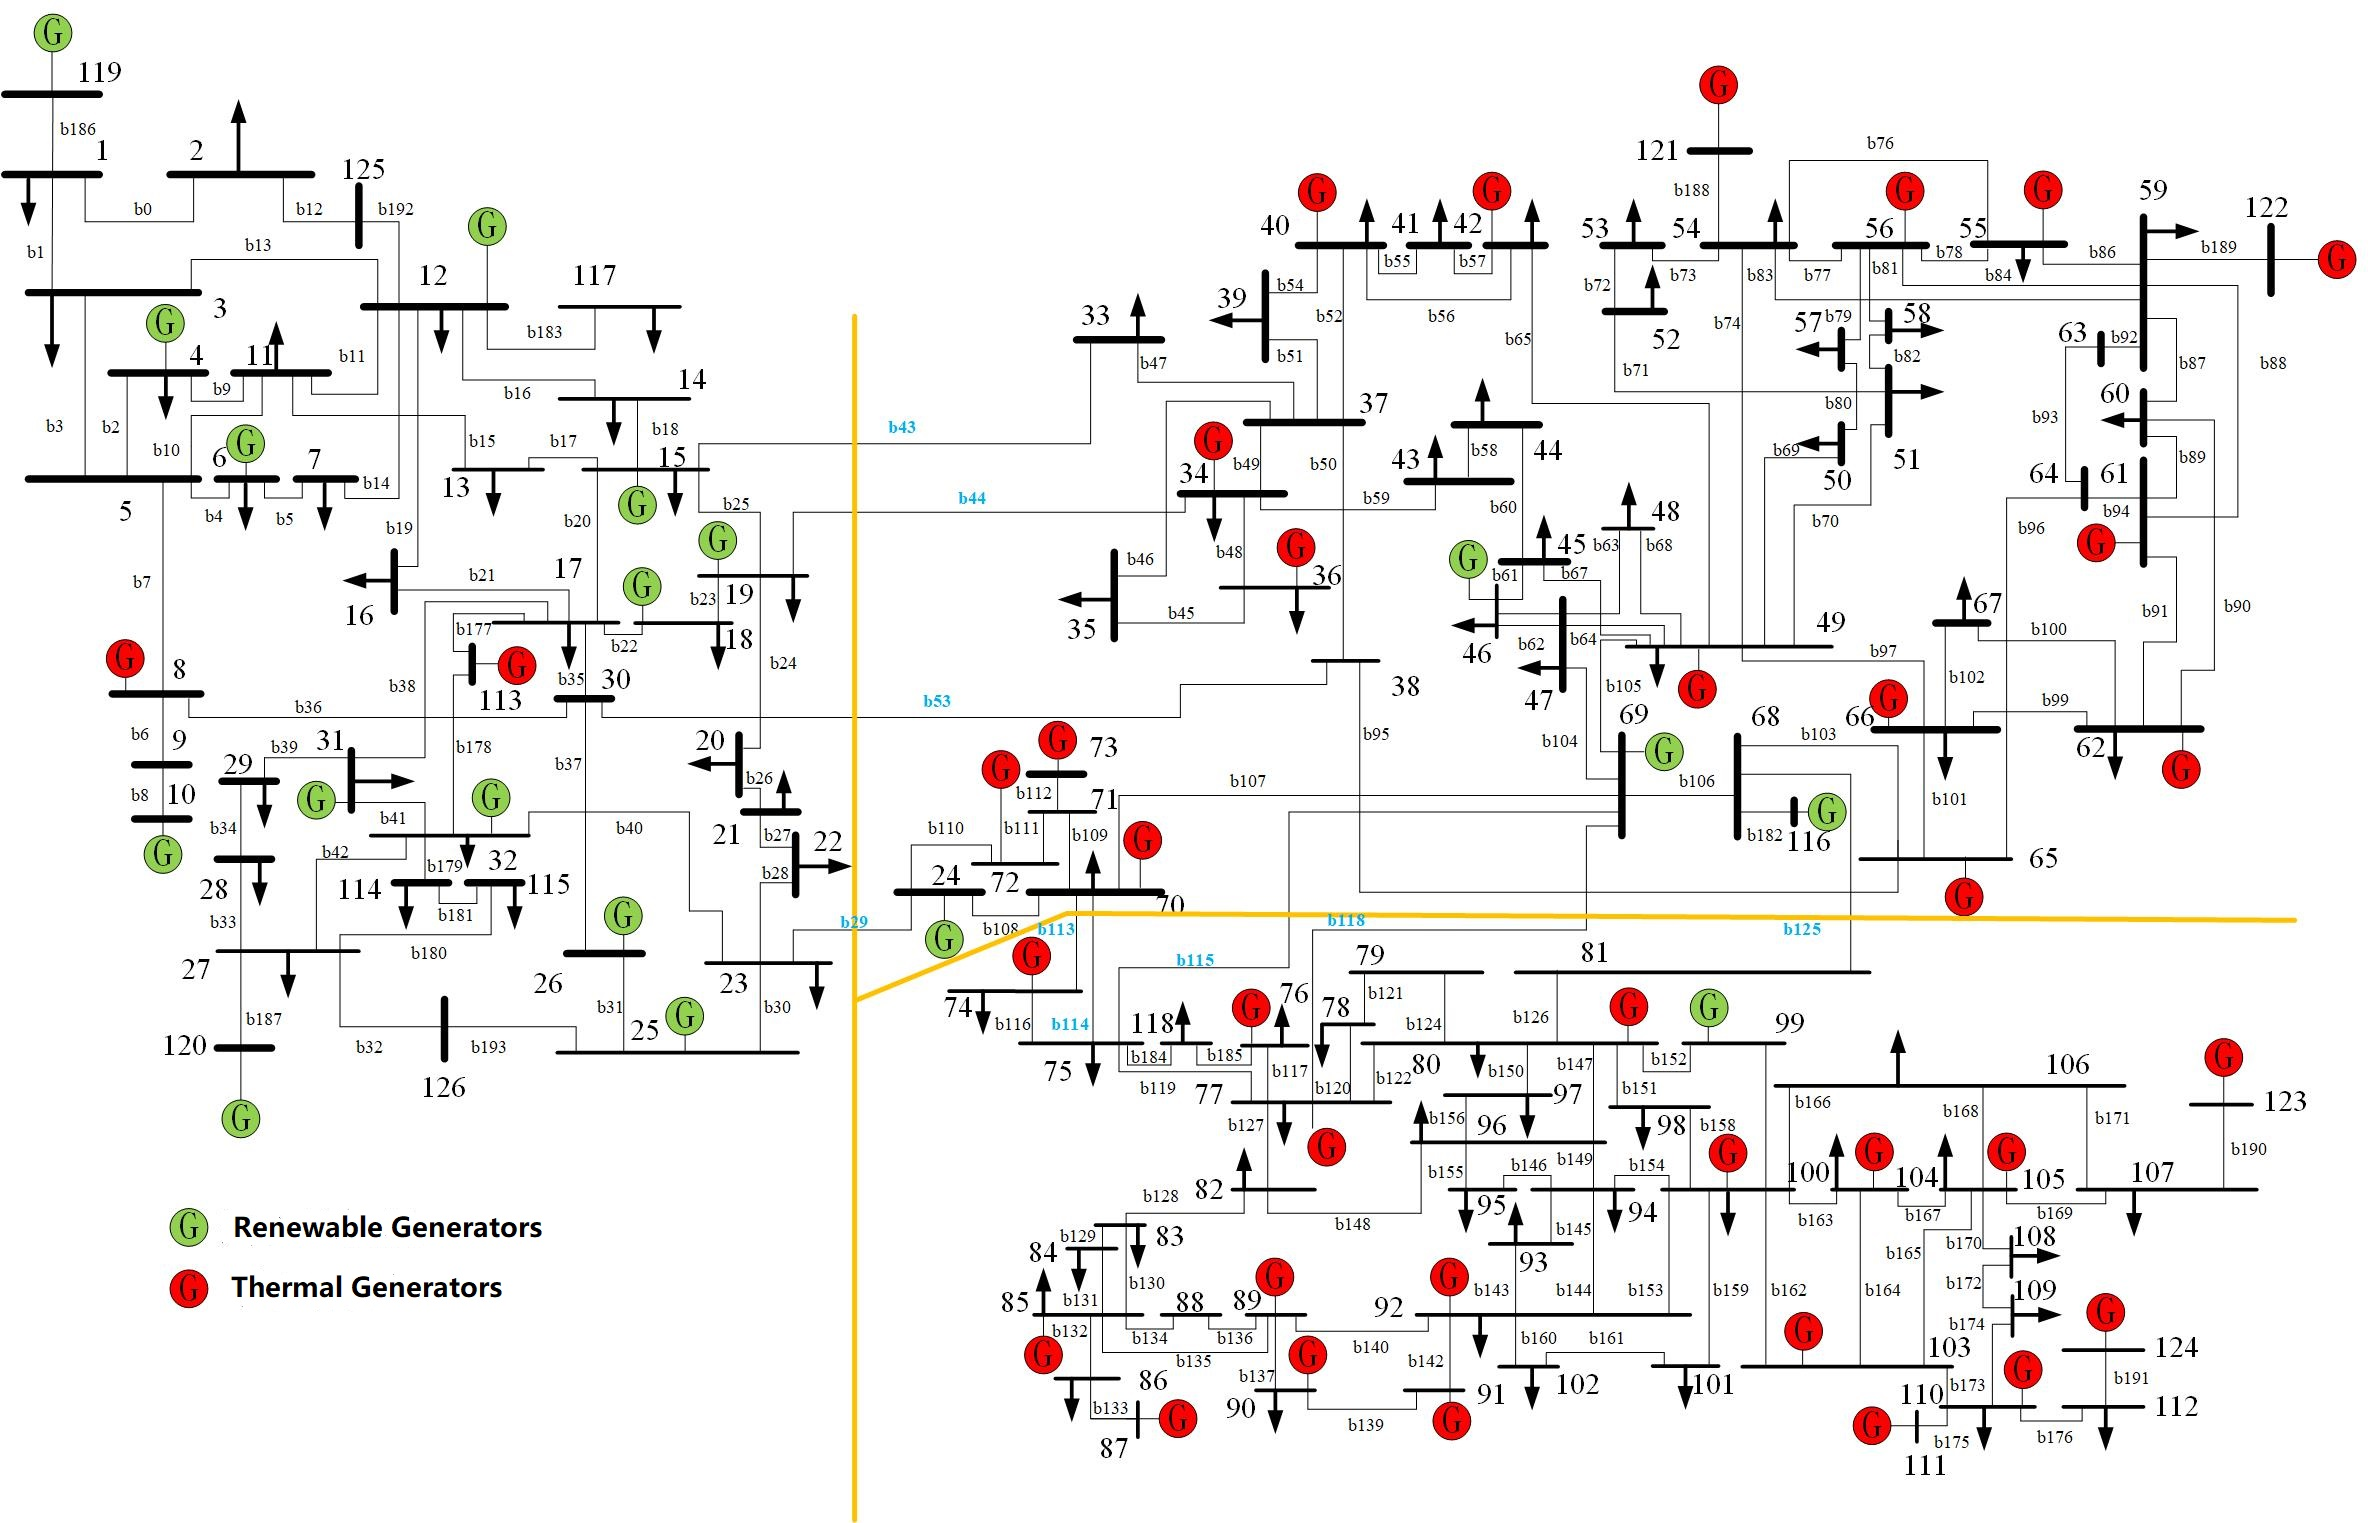
\includegraphics[width=1.0\linewidth]{fig/SG126.jpg}
    \captionsetup{labelformat=empty}
    \caption{\textbf{Extended Fig. 6:} Provincial power grid of GridSim, includes 126 buses, 185 lines, and 54 generators, 17 of which are renewable.}
    \label{fig:grid_arch}
\end{figure}

\subsubsection*{Hyperparameters}
As shown in Extended Table.4, we released some hyperparameters for training settings to help researchers who are interested in GridZero better reproduce our work.
\begin{table}[h]
    \label{tab:param}
\begin{center}
\begin{small}
% \begin{sc}
\centering
\scalebox{1.0}{
\centering
\begin{tabular}{lc}
\toprule
Parameter & Setting \\
\midrule
Observation & 839 \\
Frames stacked & 1 \\
Frames skip & 0 \\
Reward clipping & True \\
Reward clipping delta & 0.1 \\
Max frames per episode & 288 \\
Discount factor & 0.99 \\
Minibatch size & 256 \\
Optimizer & SGD \\
Optimizer: learning rate & 0.01 \\
Optimizer: momentum & 0.9 \\
Optimizer: weight decay ($c$) & 2e-5 \\
Learning rate schedule & exponential, 0.5 \\
Max gradient norm & 10 \\
Priority exponent ($\alpha$) & 0.6 \\
Priority correction ($\beta$) & 0.4 \\
Training steps & 100k \\
Self-play network updating inerval & 100 \\ 
Target network interval & 200 \\
Unroll steps ($l_{\text{unroll}}$) & 5 \\
TD steps ($k$) & 5 \\
Policy loss coefficient ($\lambda_1$) & 1 \\
Value loss coefficient ($\lambda_2$) & 0.5 \\
Reward loss coefficient ($\lambda_3$) & 1.0 \\
Self-supervised consistency loss coefficient ($\lambda_4$) & 2.0 \\
Dirichlet noise alpha ($\xi$) & 0.3 \\
Dirichlet noise ratio & 0.25 \\
Number of simulations in MCTS ($N_{\text{sim}}$) & 50 \\
Number of sampled normal actions & 13 \\
Number of sampled actions with small noises & 2 \\
Number of sampled actions with bigger noises & 2 \\
Reanalyzed ratio & 1.0 \\
\bottomrule
\end{tabular}
}
\end{small}
\end{center}
\captionsetup{labelformat=empty}
    \caption{\textbf{Extended Table. 4:} Hyper-parameters for GridZero}
\end{table}




